\section{Acquired Knowledge} %is this good?..

\textcolor{red}{Some introductory info.}

\subsection{Studying dsPICs}

\textcolor{red}{Some theoretical knowledge.
Something like listing a short summary of everything we've studied. }

\subsection{Fusion}

\subsubsection{Fusion Workshop}
For learning Autodesk Fusion 360, a one-day workshop was held. In this workshop, the basic aspects of CAD modelling and basic features of Fusion 360 were introduced, as well as more advanced features such as history timeline, version control, and collaboration between users.

One very helpful thing that we learned in the workshop is to import 3rd party parts. The 3D model of the motor that we are using is imported, such that a fitting motor mount can be designed very precisely and accurately according to the dimension of the motor. (Fig. \ref{fig:fusion_import})

We practiced using many “modeling” features, as well as “assembly” features such as joint, and changing “physical material” and “appearance” to create a box with a moving joint that can be opened and has varying appearances. Later the user collaboration feature was demonstrated using these boxes by assembling them on a table. (Fig. \ref{fig:fusion_collab_table})

\begin{figure}[htb]
    \centering
    \begin{minipage}[b]{0.4\textwidth}
    	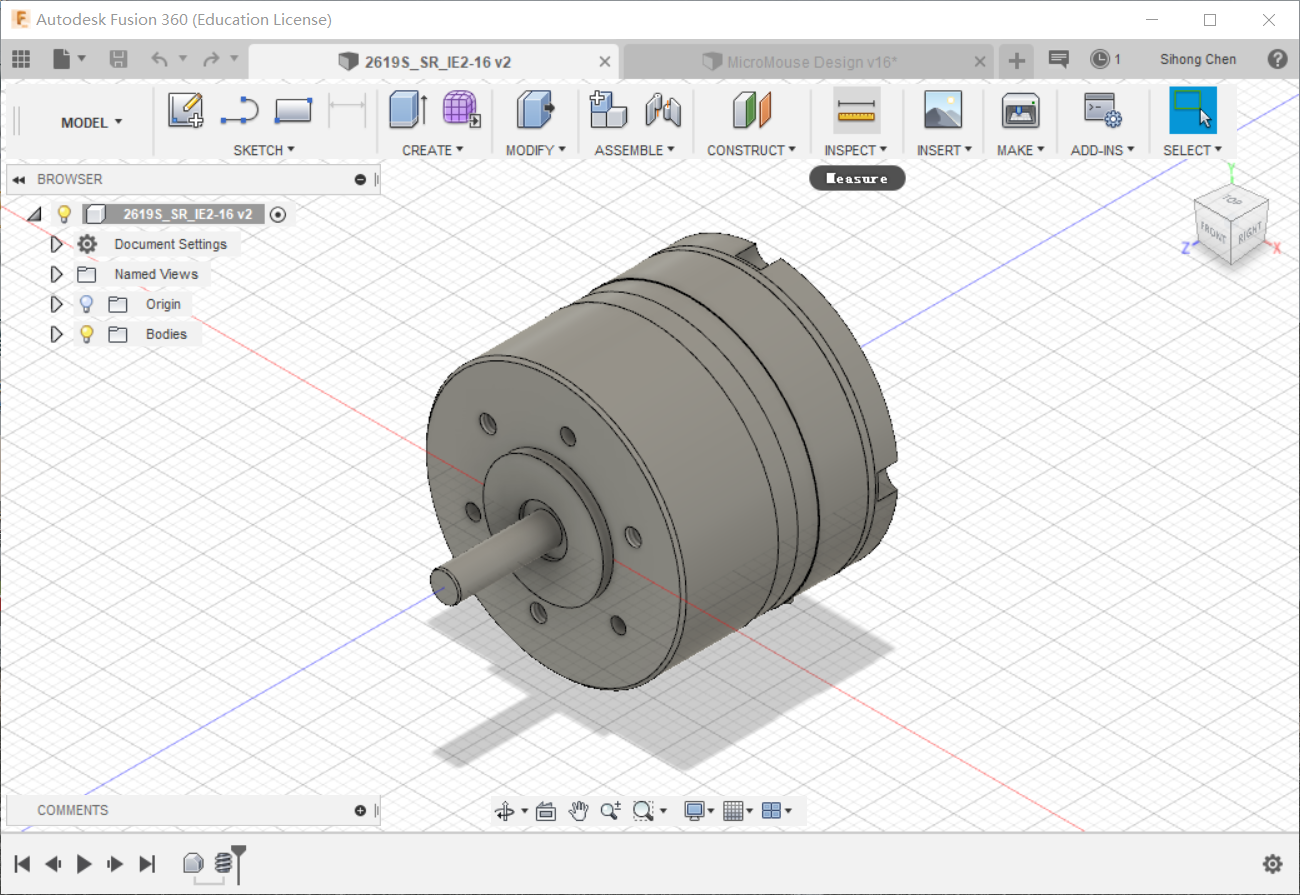
\includegraphics[width=\textwidth]{figures/Casing/FusionImport.png}
    	\caption{Import 3D CAD Model from 3rd party}
    	\label{fig:fusion_import}
  	\end{minipage}
 
  	\begin{minipage}[b]{0.4\textwidth}
  	  includegraphics[width=textwidth]{figures/Casing/FusionCollaborationTable.png}
  	  \caption{Individually made boxes put together on one table in Fusion collaboration}
  	  \label{fig:fusion_collab_table}
  	\end{minipage}
\end{figure}

In the workshop, a synchronisation feature between Autodesk EAGLE and Autodesk Fusion 360 is briefly introduced, which has the potential to reduce the back-and-forth process between CAD 3D model design and PCB design. However, in practice, we find that the lack of 3D models from the electronic components that we are using renders the usefulness of this feature somewhat limited.

\subsubsection{Further learning}
In order to tackle some of the challenges we faced for designing the casing, some more advanced features of Fusion 360 have been utilised.

One example is to set “parameter” values when creating the parts, which allowed easy modification to the model. This is helpful because our design processes are parallel to each other, and in the end the casing has to matched the physical dimension of the board. Therefore a back-and-forth process between PCB design and CAD design is unavoidable. The “parameter” feature in Fusion 360 accelerates this process and saves a lot of time and unnecessary work.

Furthermore the freeform and sculpting tool enables us to create more free flowing surfaces. This tool is traditionally reserved for industrial designers, and by combining this with the CAD solid modelling environment, Fusion 360 has partially earned its namesake: a fusion of different design processes. For our project, it enabled a more interesting look to the design.

\FloatBarrier
\vspace{1cm}

\subsection{Eagle}

\textcolor{red}{Not sure if we should mention it here, but why not.
\linebreak
\textbf{your suggestions for other subsections are highly appreciated}}
